\problem{}
\subproblem{}
قضیه حد مرکزی:
فرض کنیم دنباله‌ای از متغیرهای تصادفی مستقل و هم توزیع (i.i.d) را داشته باشیم،
 که به صورت \( X_1, X_2, \ldots, X_n \) نشان داده می‌شوند. قضیه حد مرکزی بیان می‌کند که توزیع متغیر تصادفی 
\[ \frac{\bar{X} - \mu}{\frac{\sigma}{\sqrt{n}}} \]
به توزیع متغیر تصادفی نرمال استاندارد نزدیک و نزدیک‌تر می‌شود وقتی که مقدار \( n \) 
به خوبی زیاد شود. به صورت رسمی، این قضیه به صورت زیر بیان می‌شود:
\[ lim_{{n \to \infty}} P\left(\frac{\bar{X} - \mu}{\frac{\sigma}{\sqrt{n}}} \leq x\right) = \Phi(x) \]
که در این‌جا \( \Phi(x) \) تابع توزیع متغیر تصادفی نرمال استاندارد است.\\
\subproblem{}
کد پایتون:\\
\begin{figure}[H]
	\centering
	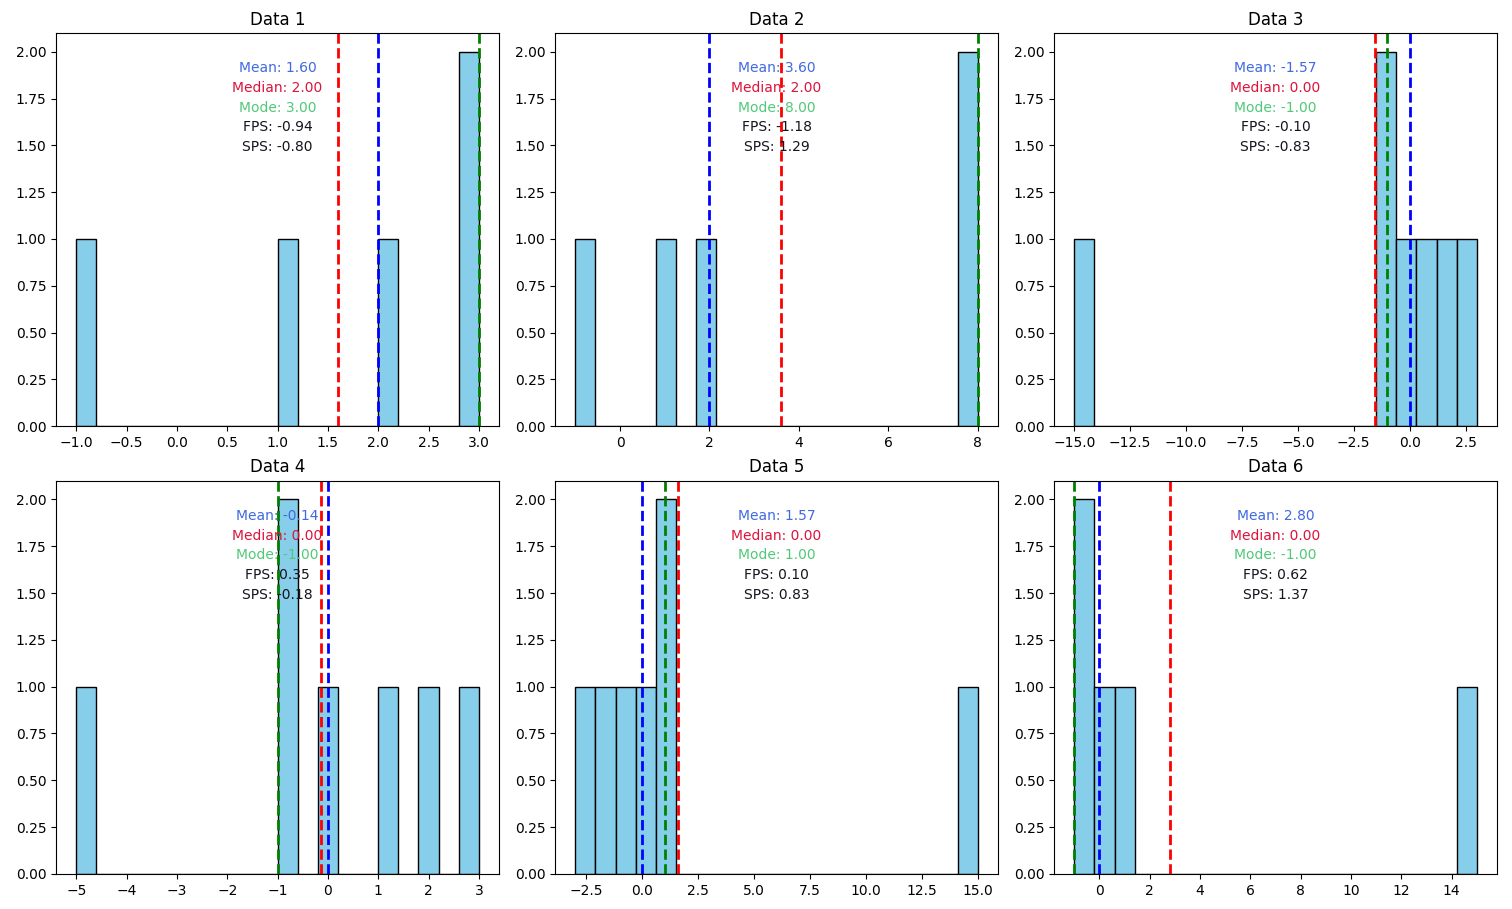
\includegraphics[width=0.5\textwidth]{/Users/kajal/Documents/statistics/resources/hw2/Figure_2.png}
\end{figure}
خروجی:\\
\begin{figure}[H]
	\centering
	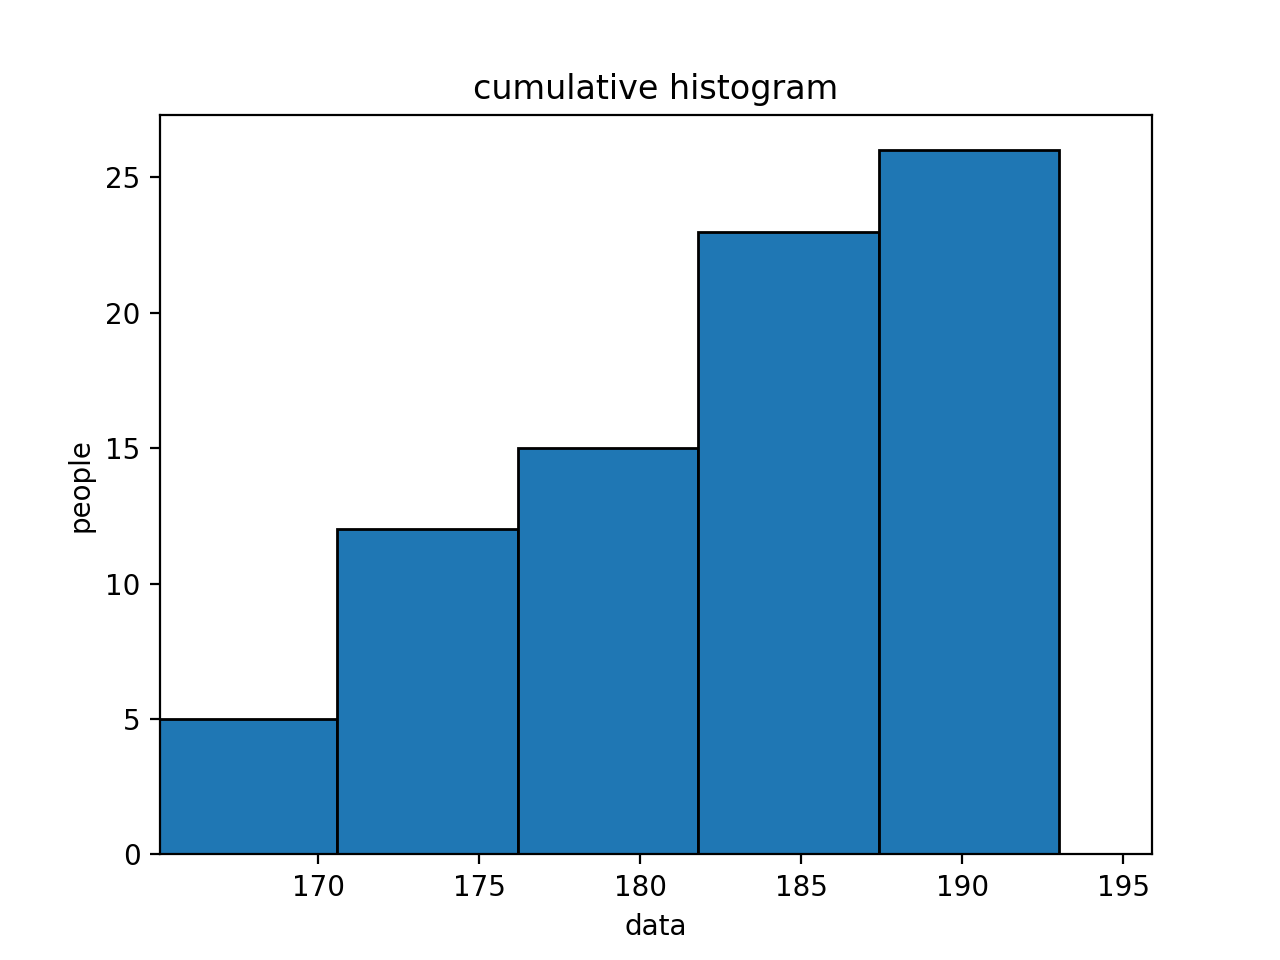
\includegraphics[width=0.5\textwidth]{/Users/kajal/Documents/statistics/resources/hw2/Figure_1.png}
\end{figure}
% \begin{lstlisting}[caption={Python Code Example}, label={lst:python}]
%     # Example Python code
%     import numpy as np
%     import matplotlib.pyplot as plt
    
%     # Generate data
%     x = np.linspace(0, 10, 100)
%     y = np.sin(x)
    
%     # Plot data
%     plt.plot(x, y)
%     plt.xlabel('x')
%     plt.ylabel('sin(x)')
%     plt.title('Plot of sin(x)')
%     plt.grid(True)
%     plt.show()
% \end{lstlisting}
